\documentclass{llncs}
\usepackage{amsmath, amssymb, fancyvrb, multirow, color, stmaryrd}
\usepackage{svg}
\usepackage{wrapfig}
\usepackage{graphicx}
\usepackage{fancyvrb}
\usepackage{hyperref}
\usepackage{framed}
\usepackage[]{algorithm2e}

\newcommand{\enforce}{\mathsf{enforce}}
\newcommand{\traj}{\mathsf{traj}}
\newcommand{\drh}{\textsf{drh}}
\newcommand{\dReal}{\textsf{dReal}}
\newcommand{\dReach}{\textsf{dReach}}

%\usepackage{multirow}
\usepackage{amsmath,hyperref}
\hypersetup{
    colorlinks,%
    citecolor=blue,%
    filecolor=blue,%
    linkcolor=blue,%
    urlcolor=blue
}
\usepackage{amssymb,verbatim}
\usepackage{fix2col,listings,fancyvrb}
\usepackage{multicol}
\usepackage{graphicx,epsfig}
\usepackage{caption}
\usepackage{stmaryrd}
\usepackage{setspace}
\usepackage{ulem}
\usepackage{newlfont}
\usepackage{epsfig,graphics}
\usepackage{fancybox}
\usepackage{listings}
\usepackage{caption}
\usepackage{graphicx,epsfig}
\usepackage{caption}
\usepackage{makeidx}
\usepackage{algorithm}
\usepackage{algpseudocode}
\usepackage{listings}
\lstset{
  basicstyle=\ttfamily,
  breaklines=true,
  columns=fullflexible,
  escapeinside = ||,
  breakindent=0pt}
\makeindex

\usepackage{algorithm}
\usepackage{algpseudocode}
\usepackage{hyperref}
\hypersetup{
    colorlinks,%
    citecolor=blue,%
    filecolor=blue,%
    linkcolor=blue,%
    urlcolor=blue
}
\usepackage{multicol}
\usepackage{lipsum}

\newtheorem{theorem}{Theorem}
\newtheorem{proofoutline}[theorem]{Proof Outline}
\newtheorem{lemma}[theorem]{Lemma}
\newtheorem{claim}[theorem]{Claim}
\newtheorem{proposition}[theorem]{Proposition}
\newtheorem{corollary}[theorem]{Corollary}
\newtheorem{fact}[theorem]{Fact}
\newtheorem{definition}[theorem]{Definition}
\newtheorem{remark}[theorem]{Remark}
\newtheorem{conjecture}[theorem]{Conjecture}
\newtheorem{example}[theorem]{Example}
\newtheorem{notation}[theorem]{Notation}
\newtheorem{question}[theorem]{Question}



%\usepackage[ruled,lined,boxed,commentsnumbered,linesnumbered]{algorithm2e}

\setcounter{secnumdepth}{3}
\setcounter{tocdepth}{2}

\newcommand\bookepigraph[4]{
\vspace{1em}\hfill{}\begin{minipage}{#1}{\begin{spacing}{0.9}
\small\noindent\textit{#2}\end{spacing}
\vspace{1em}
\hfill{}{#3}\\

\vspace{-1em}\begin{flushright}{#4}\end{flushright}}\vspace{2em}
\end{minipage}}

\newcommand{\dom}{\mbox{dom}}

\newcommand\epigraph[3]{
\vspace{1em}\hfill{}\begin{minipage}{#1}{\begin{spacing}{0.9}
\small\noindent\textit{#2}\end{spacing}
\vspace{1em}
\hfill{}{#3}}\vspace{2em}
\end{minipage}}

\newcommand\anonymousepigraph[2]{
\vspace{1em}\hfill{}\begin{minipage}{#1}{\begin{spacing}{0.9}
\small\noindent\textit{#2}\end{spacing}}
\vspace{1em}
\end{minipage}}

\newcommand{\len}{\mathit{len}}
\newcommand{\poly}{\mathsf{poly}}
\newcommand{\N}{\mathbb{N}}
\newcommand{\R}{\mathbb{R}}
\newcommand{\D}{\mathbb{D}}
\newcommand{\cf}{\mathsf{CF}}
\newcommand{\be}{\mathsf{BE}}
\newcommand{\fe}{\mathbb{F}^{[\underline{e}, \overline{e}]}_{\beta,p}}
\newcommand{\rad}{\mathrm{rad}}


\newcommand{\flow}{\mathsf{flow}}
\newcommand{\jump}{\mathsf{jump}}
\newcommand{\inv}{\mathsf{inv}}
\newcommand{\init}{\mathsf{init}}
\newcommand{\guard}{\mathsf{guard}}
\newcommand{\reset}{\mathsf{reset}}
\newcommand{\reach}{\mathsf{Reach}}
\newcommand{\unsafe}{\mathsf{unsafe}}

\newcommand{\safe}{\mathsf{safe}}
\newcommand{\p}{\mathsf{P}}
\newcommand{\np}{\mathsf{NP}}
%\newcommand{\dom}{\mathrm{dom}}


\newcommand\tupleof[1]{\left\langle #1 \right\rangle}
\newcommand\vI{\vec{I}}
\newcommand\va{\vec{a}}
\newcommand\vb{\vec{b}}
\newcommand\vc{\vec{c}}
\newcommand\vd{\vec{d}}
\newcommand\ve{\vec{e}}
\newcommand\vl{\vec{l}}
\newcommand\vu{\vec{u}}
\newcommand\vx{\vec{x}}
\newcommand\vy{\vec{y}}
\newcommand\trp[1]{#1^{{}^{\mbox{\sc{t}}}}}
\newcommand{\lrf}{\mathcal{L}_{\mathbb{R}_{\mathcal{F}}}}
%\usepackage{wrapfigure}

%\doublespacing


\title{\dReach{}: $\delta$-Reachability Analysis\\ for Hybrid Systems}

\begin{document}


\mainmatter  % start of an individual contribution

\author{Soonho Kong, Sicun Gao, Wei Chen, and Edmund Clarke}
\authorrunning{S. Kong, S. Gao, W. Chen,  E. Clarke}
\institute{Computer Science Department, Carnegie Mellon University, USA}
\maketitle

\begin{abstract}
  \dReach{} is a bounded reachability analysis tool for nonlinear
  hybrid systems. It encodes reachability problems of hybrid systems
  to first-order formulas over real numbers, which are solved by
  delta-decision procedures in the SMT solver \dReal{}. In this way,
  \dReach{} is able to handle a wide range of highly nonlinear hybrid
  systems. It has scaled well on various realistic models
  from biomedical and robotics applications.
\end{abstract}

% Tool demonstration papers focus on the usage aspects of tools. As with
% regular tool papers, authors are strongly encouraged to make their
% tools publicly available, preferably on the web. Theoretical
% foundations and experimental evaluation are not required, however, a
% motivation as to why the tool is interesting and significant should be
% provided. Tool demonstration papers can have a maximum of 6 pages.
% They should have an appendix of up to 6 additional pages with details
% on the actual demonstration.

\section{Introduction}\label{sec:intro}

% Need a paragrapgh or two to explain why the tool is interesting and
% significant should be provided.

\dReach{} is a bounded model checker for hybrid systems. It encodes
bounded reachability problems of hybrid systems as first-order
formulas over the real numbers, and solves them using
$\delta$-decision procedures in the SMT solver \dReal{}. \dReach{} is
able to handle a wide range of highly nonlinear hybrid systems. It has
scaled well on various realistic nonlinear models from biomedical and
robotics applications~\cite{}.

It is well-known that the standard bounded reachability problems for
simple hybrid systems are already highly
undecidable~\cite{DBLP:conf/rex/AlurD91,DBLP:conf/hybrid/AlurCHH92}. In
previous work~\cite{}, we have defined the notion of
$\delta$-reachability problem of hybrid systems. In this new
framework, we have shown that bounded $\delta$-reachability is
decidable for a wide range of hybrid systems, with reasonable
complexity bounds~\cite{}. We give a brief review of the framework in
Section~\ref{sec:delta-reachability}.

Realistic hybrid systems involves nonlinear ODEs with transcendental
functions. \dReach{} allows users to specify a hybrid system in a
nonlinear signature as it is without linearizing or overapproximating
it. Users can provide the tool with a numerical error bound $\delta$,
a bounded time horizon $[0, T]$, and a maximum number of mode switches
$k$ for the analysis. As a result of analysis, \dReach{} will return
either \textbf{$\delta$-sat} with a concrete counterexample, or
\textbf{unsat} which does not involve numerical errors. We also
provide a visualization for the $\delta$-sat case to help
understand the analysis result.
\begin{figure}[!t]
  \subfloat[An example of nonlinear hybrid system model: off-treatment
  mode of the prostate cancer treatement model~\cite{}\label{subfig-1:prostate}]{
    \includegraphics[width=0.48\textwidth]{images/prostatebw-mode2.pdf}
  }
  \hfill
  \subfloat[Visualization of a concrete counterexample generated from
  dReach for the prostate cancer treatment model.]{%
    \includegraphics[width=0.48\textwidth]{images/prostate}
  }
  \caption{An example of nonlinear hybrid system model: Prostate
    cancer model.}
  \label{fig:prostate-example}
\end{figure}
For instance, figure~\ref{fig:prostate-example} shows a part of a
prostate cancer treatment model that contains nonlinear ODEs and a
visualization of a generated concrete counterexample.

\paragraph{Related Work}
%reachable set computation tools: flow star, SpaceX, Phaver,
%theorem provers:
%similar tools: iSAT, RSolver -- emphasize on the nonlinearity that we can handle.

The paper is structured as follows.


%%% Local Variables:
%%% mode: latex
%%% TeX-master: "main"
%%% End:

\section{System Description}

\begin{figure}
  \centering
  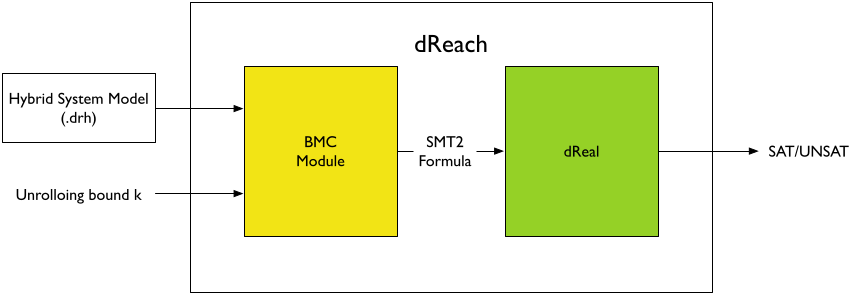
\includegraphics[width=\textwidth]{images/dReach}
  \caption{System Description of \dReach{}}
  \label{fig:system-description}
\end{figure}

Figure~\ref{fig:system-description} illustrates the architecture of
\dReach{}. We provide a domain-specific lanaguage to describe a hybrid
system and specify its safety properties. Given an input model,
specification, and unrolling bound $k$, \dReach{} reduces the
$\delta$-reachability problem to a $\delta$-decision problem of
formulas over the reals by providing a corresponding SMT encoding for
the problem. Then we answer the bounded reachability queries by using
our nonlinear SMT solver \dReal{}~\cite{DBLP:conf/cade/GaoKC13} to
solve the encoded problems.

\subsection{drh: a Language for Modeling and Specifying Hybrid Systems}

We define \texttt{drh}, a small language for describing hybrid systems
and specifying their initial and safety conditions. It consists of
five sections - macro definitions, variable declarations, mode
definitions, and initial condition, and goals.
\begin{align*}
  \textit{drh} := \ & \textit{macro-definition}^*\\
                  & \textit{variable-declaration}^+\\
                  & \textit{mode-definition}^+\\
                  & \textit{initial-condition}\\
                  & \textit{goal}^+
\end{align*}
In macro definitions, we allow users to define C-preprocessor macros
which can be used in following sections. Macros are expanded before
the other parts are processed.

A variable declaration has a form:
\[
\textit{variable-declaration} \ := \ \texttt{[}
                                     \textit{l}
                                     \texttt{,}
                                     \ \textit{u}
                                     \texttt{]}
                                     \ \textit{var}
                                     \texttt{;}
\]
and it declares a real variable $var$ whose domain is $[l, u] \in
\mathbb{IR}$. A special variable \textit{time} has to be delcared to
specify the time bound of bounded model checking.

A mode definition consists of mode id, mode invariant, flow, and jump.
\begin{align*}
  \textit{mode-definition} \ := & \ \texttt{\{}
                                    \texttt{mode} \ \textit{id}\texttt{;}\\
                           & \ \ \  \texttt{invt}:(\textit{formula} \texttt{;})^+\\
                           & \ \ \  \texttt{flow}:\textit{ode}^+\\
                           & \ \ \ \texttt{jump}:\textit{jump}^+ \texttt{\}}
\end{align*}
\textit{id} is a unique unsigned integer assigned to a mode. An
invariant is a conjuction of logic formulae which must hold in a mode.
A flow describes a continuous dynamics of a mode by providing a set of
ordinary differential equations (\textit{ode}s) which is a form of
``\texttt{d/dt[}\textit{x}\texttt{]=}\textit{exp}''. \textit{jump} is
a form of ``\textit{guard} \texttt{==>} \texttt{@}\textit{n}
\textit{reset}'' where \textit{guard} is a logic formula specifying a
condition to make a transition, $n$ is an id of target mode, and
\textit{reset} is a logic formula specifying the relationship between
old and new values.

\texttt{initial-condition} is of a form
``\texttt{@}\textit{mode-id} \textit{formula}\texttt{;}''
where \textit{mode-id} is an initial mode of a hybrid system and
\textit{formula} specifies the initial configuration of it.

\texttt{goal} shares the same syntactic structure,
``\texttt{@}\textit{mode-id} \textit{formula}\texttt{;}'' of
\textit{initial-condition} with a different interpretation. It poses a
reachability question: ``Is there a trajectory of a hybrid system
reaching \textit{mode-id} while satisfying the goal condition \textit{formula}?''.

\subsection{Encoding Bounded Reachability Problem}
\subsubsection{Encoding}
There are different encodings according to the requirements of the
solution. Out encoding formula is described in
\cite{gao2014delta}. The critical definitions that are related are
listed as follows:

\begin{definition}
Let $H$ be a hybrid automaton. We use $\unsafe = \{\unsafe_q:q\in Q\}$
in the state space of $H$. We can write $\llbracket \unsafe\rrbracket
= \bigcup_{q\in Q} \llbracket \unsafe_q \rrbracket\times \{q\}$.
\end{definition}

\begin{definition}
Let $Q = \{q_1,...,q_m\}$ be a set of modes. For any $q\in Q$, and
$i\in\mathbb{N}$, use $b_{q}^i$ to represent a Boolean variable. We
now define
$$\enforce_Q(q,i) = b^i_{q} \wedge \bigwedge_{p\in Q\setminus\{q\}}\neg b^{i}_{p}$$
$$\enforce_Q(q, q',i) = b^{i}_{q}\wedge \neg b^{i+1}_{q'} \wedge
\bigwedge_{p\in Q\setminus\{q\}} \neg b^i_{p} \wedge \bigwedge_{p'\in
  Q\setminus\{q'\}} \neg b^{i+1}_{p'}$$ We omit the subscript $Q$ when
the context is clear.
\end{definition}

\begin{definition}[$k$-Step Reachability, Invariant-Free Case]
Suppose $H$ is invariant-free, and $U$ a subset of its state space
represented by $\unsafe$. The $\lrf$-formula $\reach_{H,U}(k,M)$ is
defined as:
\begin{eqnarray*}
%\reach^{k,M}(H,U) &:=&
& &\exists^X \vec x_{0} \exists^X\vec x_{0}^t\cdots \exists^X \vec
  x_{k}\exists^X\vec x_{k}^t\exists^{[0,M]}t_0\cdots
  \exists^{[0,M]}t_k.\\ & &\bigvee_{q\in Q} \Big(\init_{q}(\vec
  x_{0})\wedge \flow_{q}(\vec x_{0}, \vec x_{0}^t, t_0)\wedge
  \enforce(q,0)\Big)\\%\wedge (b_{q_i}\wedge \bigwedge_{q\neq q_i}
  \neg b_{q}) \wedge & & \bigwedge_{i=0}^{k-1}\bigg( \bigvee_{q, q'\in
    Q} \Big(\jump_{q\rightarrow q'}(\vec x_{i}^t, \vec x_{i+1})\wedge
  \enforce(q,q',i)\\ & & \hspace{4.7cm}\wedge\flow_{q'}(\vec x_{i+1},
  \vec x_{i+1}^t, t_{i+1})\wedge \enforce(q',i+1)\Big)\bigg)\\ \wedge
  & & \bigvee_{q\in Q} \unsafe_q(\vec x_{k}^t).
\end{eqnarray*}
\end{definition}

%%% Local Variables:
%%% mode: latex
%%% TeX-master: "main"
%%% End:

\section{Logical Encoding of Reachability}


The details of our encoding scheme is given in~\cite{DBLP:journals/corr/GaoKCC14}. 
Here we focus on explaining how differential equations and the universal quantifications 
generated by mode invariance conditions are encoded, as an extension of the SMT-LIB
~\cite{BarST-SMT-10} standard. Although such formulas are automatically generated by \dReach{}
from the hybrid system descrpition, the explanation below can be helpful for 
understanding the inner mechanism of our solver. 

\paragraph{Encoding integrations.}
In each mode of a hybrid system, we need to specify continuous flows defined 
by systems of ordinary differential equations. We extend SMT-LIB with a command
\texttt{define-ode} to define such systems. For instance, we use $\texttt{define-ode}$ as follows to
assign a name $\mathrm{flow_1}$ to a group of ODE,
$\frac{\mathrm{d}x}{\mathrm{d}t} = v$ and
$\frac{\mathrm{d}v}{\mathrm{d}t} = -9.8$.
\[
\texttt{(define-ode flow\_1 ((= d/dt[x] v) (= d/dt[v] -9.8)))}
\]
We then allow integration terms in the formula. We view the solution of system of differential equations 
as a constraint between the initial-state variables, time duration, and the end-state variables. We can then naturally write
\[
\texttt{(integral 0 t [x\_0\_0 x\_0\_1 ... x\_0\_n] flow\_i)}.
\]
Note that we do not include a variable in $\vec{x}^t$ such as
\texttt{x\_t\_n} because it can be inferred from the given time
\texttt{t} and $\vec{x}^0$ variables (such as \texttt{x\_0\_n}).

\paragraph{Universal quantification for mode invariant constriants.} To encode mode invariants in hybrid systems, we
need $\exists\forall^t$-formulas~\cite{DBLP:conf/fmcad/GaoKC13} which
is a restricted form of $\exists\forall$ formula where the universal
quantifications are limited to the time variables. In \drh{}, we
introduce a new keyword $\texttt{forall\_t}$ to encode
$\exists\forall^t$ formulas. Given a time bound $[0, time_i]$, mode
invariant f at mode $n$ is encoded into \texttt{(forall\_t n [0
  time\_i] f)}.

%%% Local Variables:
%%% mode: latex
%%% TeX-master: "main"
%%% End:

\section{Using \dReach{}}\label{sec:using-dreach}

We now describe the input format and command line options of \dReach{}. 

\subsection{Input Format}\label{sec:input-format}

We now describe the input language for describing hybrid systems and
specifying reachability properties. It consists of five sections
- macro definitions, variable declarations, mode definitions, and
initial condition, and goals.
\begin{align*}
  \textit{drh} := \ & \textit{macro-definition}^*\\
                    & \textit{variable-declaration}^+\\
                    & \textit{mode-definition}^+\\
                    & \textit{initial-condition}\\
                    & \textit{goal}^+
\end{align*}
In macro definitions, it allows users to define macros in C
preprocessor (\texttt{cpp}) style which can be used in the following
sections. Note that macro expansions occur before the other parts are processed.

A variable declaration has a form:
\[
\textit{variable-declaration} \ := \ \texttt{[}
                                     \textit{l}
                                     \texttt{,}
                                     \ \textit{u}
                                     \texttt{]}
                                     \ \textit{var}
                                     \texttt{;}
\]
and it declares a real variable, $var$ and its domain $[l, u]$ which
is in Real interval $\mathbb{IR}$. It requires a special variable
declaration for \textit{time}, to specify the upperbound of time
duration in the analysis of bounded $\delta$-reachability.

A mode definition consists of mode id, mode invariant, flow, and jump.
\begin{align*}
  \textit{mode-definition} \ := & \ \texttt{\{}
                                    \texttt{mode} \ \textit{id}\texttt{;}\\
                           & \ \ \  \texttt{invt}:(\textit{formula} \texttt{;})^+\\
                           & \ \ \  \texttt{flow}:\textit{ode}^+\\
                           & \ \ \ \texttt{jump}:\textit{jump}^+ \texttt{\}}
\end{align*}
\textit{id} is a unique positive interger assigned to a mode. An
invariant is a conjuction of logic formulae which must always hold in
a mode. A flow describes a continuous dynamics of a mode by providing
a set of ordinary differential equations (\textit{ode}s) which is a
form of
``\texttt{d/dt[}\textit{x}\texttt{]=}\textit{exp}''. \textit{jump} is
a form of ``\textit{guard} \texttt{==>} \texttt{@}\textit{n}
\textit{reset}'' where \textit{guard} is a logic formula specifying a
condition to make a transition, $n$ denotes the target mode-id, and
\textit{reset} is a logic formula connecting the old and new values
for the transition.

\texttt{initial-condition} is of a form
``\texttt{@}\textit{mode-id} \textit{formula}\texttt{;}''
where \textit{mode-id} is an initial mode of a hybrid system and
\textit{formula} specifies the initial configuration of it.

\texttt{goal} shares the same syntactic structure,
``\texttt{@}\textit{mode-id} \textit{formula}\texttt{;}'' of
\textit{initial-condition} with a different interpretation. It poses a
reachability question: ``Is there a trajectory of a hybrid system
reaching \textit{mode-id} while satisfying the goal condition \textit{formula}?''.

\begin{figure}
  \centering
  \begin{Verbatim}[fontfamily=courier, frame=single, framesep=1mm,
  numbers=left, fontsize=\scriptsize]
#define D 0.45
#define K 0.9
[0, 15] x;
[9.8] g;
[-18, 18] v;
[0, 3] time;
{   mode 1;
    invt: (v <= 0);  (x >= 0);
    flow: d/dt[x] = v;
          d/dt[v] = -g - (D * v ^ 2);
    jump: (x = 0) ==> @2 (and (x' = x) (v' = - K * v)); }
 {  mode 2;
    invt: (v >= 0); (x >= 0);
    flow: d/dt[x] = v;
          d/dt[v] = -g + (D * v ^ 2);
    jump: (v = 0) ==> @1 (and (x' = x) (v' = v)); }
init: @1 (and (x >= 5) (v = 0));
goal: @1 (and (x >= 0.45));
\end{Verbatim}
\caption{An example of \drh{} format: Inelastic bouncing ball with air
  resistance. At lines 1 and 2, we define a drag coefficient $D = 0.45$
  and an elastic coefficient $K = 0.9$ using \texttt{\#define} macros.
  At lines 3 - 6, we declare variables $x, g, v,$ and $time$. At lines
  7 - 15 and 16 - 24, we define two modes -- the falling and the
  bouncing-back modes respectively. At lines 25 and 26, we specify
  that this hybrid system starts at mode 1 (\texttt{@1}) with initial
  condition satisfying $x \ge 5 \land v = 0$. At lines 28 and 29, it
  is asking whether we can have a trajectory ending at mode 1
  (\texttt{@1}) while the height of the ball is higher than $0.45$.}
\label{fig:bouncing-ball-drh}
\end{figure}

Figure~\ref{fig:bouncing-ball-drh} shows a canonical example of hybrid
systems, an inelastic bouncing ball with air resistance, in \drh{}
format.

%%% Local Variables:
%%% mode: latex
%%% TeX-master: "main"
%%% End:
\subsection{Command Line Options}
  \begin{Verbatim}[fontfamily=courier, frame=single, framesep=1mm, fontsize=\scriptsize]
usage: /home/soonhok/work/dreal/bin/dReach options <*.drh> <options to dReal>

dReach: Bounded Model Checking for for Nonlinear Hybrid Systems

OPTIONS:
   -k   unrolling steps  (default: 3)
   -b   use BMC heuristic with disjunctive path encoding
   -r   -b and filter unreachable modes from SMT encoding
   -e   -r and filter continuous variables from SMT encoding
   -d   disjunctive path encoding

EXAMPLE:

   dReach -k 10 bouncing_ball.drh --verbose --precision=0.001 --visualize

\end{Verbatim}

\begin{figure}
  \centering
  \includegraphics[width=\textwidth]{images/cardiac}
  \caption{Visualization of $\delta$-reachable trajectory for
    a cardiac-cell model.}
  \label{fig:viz}
\end{figure}


%%% Local Variables:
%%% mode: latex
%%% TeX-master: "main"
%%% End:

\section{Example: Inelastic Bouncing Ball with Drag}
\begin{wrapfigure}{l}{0.5\textwidth}
  \centering
  \includegraphics[width=0.5 \textwidth]{images/bouncing_ball.pdf}
  \caption{Bouncing ball example}
  \label{fig:bouncing-ball}
\end{wrapfigure}


\begin{figure}
  \centering
  \begin{Verbatim}[fontfamily=courier, frame=single, framesep=1mm,
  numbers=left, fontsize=\scriptsize]
#define D 0.45
#define K 0.9
[0, 15] x;
[9.8] g;
[-18, 18] v;
[0, 3] time;
{
  mode 1;
  invt:
        (v <= 0);
        (x >= 0);
  flow:
        d/dt[x] = v;
        d/dt[v] = -g + (- D * v ^ 1);
  jump:
        (x = 0) ==> @2 (and (x' = x) (v' = - K * v));
}
{
  mode 2;
  invt:
        (v >= 0);
        (x >= 0);
  flow:
        d/dt[x] = v;
        d/dt[v] = -g + (- D * v ^ 1);
  jump:
        (v = 0) ==> @1 (and (x' = x) (v' = v));
}
init:
@1    (and (x >= 5) (v = 0));

goal:
@1    (and (x >= 0.45));
\end{Verbatim}
  \caption{Bouncing ball example}
  \label{fig:bouncing-ball}
\end{figure}

\begin{figure}
  \centering
  \begin{Verbatim}[fontfamily=courier, frame=single, framesep=1mm,
  numbers=left, fontsize=\scriptsize]
(set-logic QF_NRA_ODE)
(declare-fun x () Real)
(declare-fun v () Real)
(declare-fun x_0_0 () Real)
(declare-fun x_0_t () Real)
...
(declare-fun x_10_0 () Real)
(declare-fun x_10_t () Real)
(declare-fun v_0_0 () Real)
(declare-fun v_0_t () Real)
...
(declare-fun v_10_0 () Real)
(declare-fun v_10_t () Real)
(declare-fun time_0 () Real)
...
(declare-fun time_10 () Real)
(declare-fun mode_0 () Real)
...
(declare-fun mode_10 () Real)
(define-ode flow_1 ((= d/dt[x] v)
                    (= d/dt[v] (+ (- 0.0 9.8) (* -0.45 (^ v 1.0))))))
(define-ode flow_2 ((= d/dt[x] v)
                    (= d/dt[v] (+ (- 0.0 9.8) (* -0.45 (^ v 1.0))))))
(assert (<= 0.0 x_0_0))
(assert (<= x_0_0 15.0))
...
(assert (<= -18.0 v_10_t))
(assert (<= v_10_t 18.0))
(assert (<= 0.0 time_0))
(assert (<= time_0 3.0))
...
(assert (<= 0.0 time_10))
(assert (<= time_10 3.0))
...

(assert (and (and (= v_0_0 0.0) (>= x_0_0 5.0)) (= mode_0 1.0) (= [x_0_t v_0_t] (integral 0. time_0 [x_0_0 v_0_0] flow_1)) (= mode_0 1.0) (forall_t 1.0 [0.0 time_0] (<= v_0_t 0.0)) (<= v_0_t 0.0) (<= v_0_0 0.0) (forall_t 1.0 [0.0 time_0] (>= x_0_t 0.0)) (>= x_0_t 0.0) (>= x_0_0 0.0) (= mode_1 2.0) (= x_0_t 0.0) (= v_1_0 (* -0.9 v_0_t)) (= x_1_0 x_0_t) (= [x_1_t v_1_t] (integral 0. time_1 [x_1_0 v_1_0] flow_2)) (= mode_1 2.0) (forall_t 2.0 [0.0 time_1] (>= v_1_t 0.0)) (>= v_1_t 0.0) (>= v_1_0 0.0) (forall_t 2.0 [0.0 time_1] (>= x_1_t 0.0)) (>= x_1_t 0.0) (>= x_1_0 0.0) (= mode_2 1.0) (= v_1_t 0.0) (= v_2_0 v_1_t) (= x_2_0 x_1_t) (= [x_2_t v_2_t] (integral 0. time_2 [x_2_0 v_2_0] flow_1)) (= mode_2 1.0) (forall_t 1.0 [0.0 time_2] (<= v_2_t 0.0)) (<= v_2_t 0.0) (<= v_2_0 0.0) (forall_t 1.0 [0.0 time_2] (>= x_2_t 0.0)) (>= x_2_t 0.0) (>= x_2_0 0.0) (= mode_3 2.0) (= x_2_t 0.0) (= v_3_0 (* -0.9 v_2_t)) (= x_3_0 x_2_t) (= [x_3_t v_3_t] (integral 0. time_3 [x_3_0 v_3_0] flow_2)) (= mode_3 2.0) (forall_t 2.0 [0.0 time_3] (>= v_3_t 0.0)) (>= v_3_t 0.0) (>= v_3_0 0.0) (forall_t 2.0 [0.0 time_3] (>= x_3_t 0.0)) (>= x_3_t 0.0) (>= x_3_0 0.0) (= mode_4 1.0) (= v_3_t 0.0) (= v_4_0 v_3_t) (= x_4_0 x_3_t) (= [x_4_t v_4_t] (integral 0. time_4 [x_4_0 v_4_0] flow_1)) (= mode_4 1.0) (forall_t 1.0 [0.0 time_4] (<= v_4_t 0.0)) (<= v_4_t 0.0) (<= v_4_0 0.0) (forall_t 1.0 [0.0 time_4] (>= x_4_t 0.0)) (>= x_4_t 0.0) (>= x_4_0 0.0) (= mode_5 2.0) (= x_4_t 0.0) (= v_5_0 (* -0.9 v_4_t)) (= x_5_0 x_4_t) (= [x_5_t v_5_t] (integral 0. time_5 [x_5_0 v_5_0] flow_2)) (= mode_5 2.0) (forall_t 2.0 [0.0 time_5] (>= v_5_t 0.0)) (>= v_5_t 0.0) (>= v_5_0 0.0) (forall_t 2.0 [0.0 time_5] (>= x_5_t 0.0)) (>= x_5_t 0.0) (>= x_5_0 0.0) (= mode_6 1.0) (= v_5_t 0.0) (= v_6_0 v_5_t) (= x_6_0 x_5_t) (= [x_6_t v_6_t] (integral 0. time_6 [x_6_0 v_6_0] flow_1)) (= mode_6 1.0) (forall_t 1.0 [0.0 time_6] (<= v_6_t 0.0)) (<= v_6_t 0.0) (<= v_6_0 0.0) (forall_t 1.0 [0.0 time_6] (>= x_6_t 0.0)) (>= x_6_t 0.0) (>= x_6_0 0.0) (= mode_7 2.0) (= x_6_t 0.0) (= v_7_0 (* -0.9 v_6_t)) (= x_7_0 x_6_t) (= [x_7_t v_7_t] (integral 0. time_7 [x_7_0 v_7_0] flow_2)) (= mode_7 2.0) (forall_t 2.0 [0.0 time_7] (>= v_7_t 0.0)) (>= v_7_t 0.0) (>= v_7_0 0.0) (forall_t 2.0 [0.0 time_7] (>= x_7_t 0.0)) (>= x_7_t 0.0) (>= x_7_0 0.0) (= mode_8 1.0) (= v_7_t 0.0) (= v_8_0 v_7_t) (= x_8_0 x_7_t) (= [x_8_t v_8_t] (integral 0. time_8 [x_8_0 v_8_0] flow_1)) (= mode_8 1.0) (forall_t 1.0 [0.0 time_8] (<= v_8_t 0.0)) (<= v_8_t 0.0) (<= v_8_0 0.0) (forall_t 1.0 [0.0 time_8] (>= x_8_t 0.0)) (>= x_8_t 0.0) (>= x_8_0 0.0) (= mode_9 2.0) (= x_8_t 0.0) (= v_9_0 (* -0.9 v_8_t)) (= x_9_0 x_8_t) (= [x_9_t v_9_t] (integral 0. time_9 [x_9_0 v_9_0] flow_2)) (= mode_9 2.0) (forall_t 2.0 [0.0 time_9] (>= v_9_t 0.0)) (>= v_9_t 0.0) (>= v_9_0 0.0) (forall_t 2.0 [0.0 time_9] (>= x_9_t 0.0)) (>= x_9_t 0.0) (>= x_9_0 0.0) (= mode_10 1.0) (= v_9_t 0.0) (= v_10_0 v_9_t) (= x_10_0 x_9_t) (= [x_10_t v_10_t] (integral 0. time_10 [x_10_0 v_10_0] flow_1)) (= mode_10 1.0) (forall_t 1.0 [0.0 time_10] (<= v_10_t 0.0)) (<= v_10_t 0.0) (<= v_10_0 0.0) (forall_t 1.0 [0.0 time_10] (>= x_10_t 0.0)) (>= x_10_t 0.0) (>= x_10_0 0.0) (= mode_10 1.0) (>= x_10_t 0.45)))
(check-sat)
(exit)
\end{Verbatim}
  \caption{Bouncing ball example}
  \label{fig:bouncing-ball}
\end{figure}

%%% Local Variables:
%%% mode: latex
%%% TeX-master: "main"
%%% End:

\bibliographystyle{abbrv}
\bibliography{tau_tacas}

\newpage
\section*{Appendix}
\newpage
\section*{Appendix: $\lrf$-Formulas and $\delta$-Decidability}

We will use a logical language over the real numbers that allows arbitrary {\em computable real functions}~\cite{CAbook}. We write $\lrf$ to represent this language. Intuitively, a real function is computable if it can be numerically simulated up to an arbitrary precision. For the purpose of this paper, it suffices to know that almost all the functions that are needed in describing hybrid systems are Type 2 computable, such as polynomials, exponentiation, logarithm, trigonometric functions, and solution functions of Lipschitz-continuous ordinary differential equations.

More formally, $\lrf = \langle \mathcal{F}, > \rangle$ represents the first-order signature over the reals with the set $\mathcal{F}$ of computable real functions, which contains all the functions mentioned above. Note that constants are included as 0-ary functions. $\lrf$-formulas are evaluated in the standard way over the structure $\mathbb{R}_{\mathcal{F}}= \langle \mathbb{R}, \mathcal{F}^{\mathbb{R}}, >^{\mathbb{R}}\rangle$. It is not hard to see that  we can put any $\lrf$-formula in a normal form, such that its atomic formulas are of the form $t(x_1,...,x_n)>0$ or $t(x_1,...,x_n)\geq 0$, with $t(x_1,...,x_n)$ composed of functions in $\mathcal{F}$. To avoid extra preprocessing of formulas, we can explicitly define $\mathcal{L}_{\mathcal{F}}$-formulas as follows.
\begin{definition}[$\lrf$-Formulas]
Let $\mathcal{F}$ be a collection of computable real functions. We define:
\begin{align*}
t& := x \; | \; f(t(\vec x)), \mbox{ where }f\in \mathcal{F} \mbox{ (constants are 0-ary functions)};\\
\varphi& := t(\vec x)> 0 \; | \; t(\vec x)\geq 0 \; | \; \varphi\wedge\varphi
\; | \; \varphi\vee\varphi \; | \; \exists x_i\varphi \; |\; \forall x_i\varphi.
\end{align*}
In this setting $\neg\varphi$ is regarded as an inductively defined operation
which replaces atomic formulas $t>0$ with $-t\geq 0$, atomic formulas $t\geq 0$
with $-t>0$, switches $\wedge$ and $\vee$, and switches $\forall$ and $\exists$.
\end{definition}
\begin{definition}[Bounded $\lrf$-Sentences]
We define the bounded quantifiers $\exists^{[u,v]}$ and $\forall^{[u,v]}$ as
$\exists^{[u,v]}x.\varphi =_{df}\exists x. ( u \leq x \land x \leq v \wedge
\varphi)$ and $
\forall^{[u,v]}x.\varphi =_{df} \forall x. ( (u \leq x \land x \leq v)
\rightarrow \varphi)$
where $u$ and $v$ denote $\lrf$ terms, whose variables only
contain free variables in $\varphi$ excluding $x$. A {\em bounded $\lrf$-sentence} is
$$Q_1^{[u_1,v_1]}x_1\cdots Q_n^{[u_n,v_n]}x_n\;\psi(x_1,...,x_n),$$
where $Q_i^{[u_i,v_i]}$ are bounded quantifiers, and $\psi(x_1,...,x_n)$ is
quantifier-free.
\end{definition}
\begin{definition}[$\delta$-Variants]\label{variants}
Let $\delta\in \mathbb{Q}^+\cup\{0\}$, and $\varphi$ an
$\lrf$-formula
$$\varphi: \ Q_1^{I_1}x_1\cdots Q_n^{I_n}x_n\;\psi[t_i(\vec x, \vec y)>0;
t_j(\vec x, \vec
y)\geq 0],$$ where $i\in\{1,...k\}$ and $j\in\{k+1,...,m\}$. The {\em
$\delta$-weakening} $\varphi^{\delta}$ of $\varphi$ is
defined as the result of replacing each atom $t_i > 0$ by $t_i >
-\delta$ and $t_j \geq 0$ by $t_j \geq -\delta$:
$$\varphi^{\delta}:\ Q_1^{I_1}x_1\cdots Q_n^{I_n}x_n\;\psi[t_i(\vec x, \vec
y)>-\delta; t_j(\vec x,
\vec y)\geq -\delta].$$
It is clear that $\varphi\rightarrow\varphi^{\delta}$~(see \cite{gao12b}).
\end{definition}
In~\cite{gao12a}, we have proved that the following $\delta$-decision problem is decidable, which is the basis of our framework.
\begin{theorem}[$\delta$-Decidability \cite{gao12a}]\label{delta-decide} Let $\delta\in\mathbb{Q}^+$ be
arbitrary. There is an algorithm which, given any bounded $\lrf$-sentence $\varphi$,
correctly returns one of the following two answers:
\begin{itemize}
\item $\delta$-$\mathsf{True}$: $\varphi^{\delta}$ is true.
\item $\mathsf{False}$: $\varphi$ is false.
\end{itemize}
When the two cases overlap, either answer is correct.
\end{theorem}
The following theorem states the (relative) complexity of the $\delta$-decision problem.
A bounded $\Sigma_n$ sentence is a bounded $\lrf$-sentence with $n$ alternating quantifier blocks 
starting with $\exists$. 
\begin{theorem}[Complexity \cite{gao12b}]\label{compmain}
Let $S$ be a class of $\lrf$-sentences, such that for any $\varphi$ in $S$, the terms in $\varphi$ are in Type 2 complexity class $\mathsf{C}$. Then, for any $\delta\in \mathbb{Q}^+$, the $\delta$-decision problem for bounded $\Sigma_n$-sentences in $S$ is in $\mathsf{(\Sigma_n^P)^C}$.
\end{theorem}
Basically, the theorem says that increasing the number of quantifier alternations will in general increase 
the complexity of the problem, unless $\mathsf{P}=\mathsf{NP}$ (recall that $\mathsf{\Sigma_0^P}=\mathsf{P}$ 
and $\mathsf{\Sigma_1^P}=\mathsf{NP}$).
This result can specialized for specific families of functions. For example, with polynomially-computable 
functions, the $\delta$-decision problem for bounded $\Sigma_n$-sentences is $\mathsf{(\Sigma_n^P)}$-complete.
For more details and results we again point the interested reader to \cite{gao12b}.

\newpage
\section*{Appendix: BCF Model in dReach}
As an example of dReach's modeling language, we report below the actual dReach file for one of 
the BCF models analyzed in the paper.

\begin{verbatim}
//Translated to drh by Sicun Gao on Apr-18-2013
// ===============================================================
// ==   Minimal Resistor Model (4 state variables)              ==
// ==                                                           ==
// ==   Author:  E. Bartocci                                    ==
// ==                                                           ==
// ==   Date:  11/05/10                                         ==
// ==                                                           ==
// ==   Free distribution with authors permission               ==
// ==                                                           ==
// ==   SUNY Stony Brook, Stony Brook, NY                       ==
// ==                                                           ==
// ===============================================================
// The following are the parameters that you can find in the paper
// A. Bueno-Orovio, M. Cherry, and F. Fenton, `Minimal model for
// human ventricular action potentials in tissue', Journal of
// Theoretical Biology, no. 253, pp. 544-560, 2008.
// ===============================================================

#define  EPI_TVP         1.4506
#define  EPI_TV1M       60.0
#define  EPI_TV2M     1150.0
#define  EPI_TWP       200.0
#define  EPI_TW1M       60.0
#define  EPI_TW2M       15.0

#define  EPI_TS1        2.7342
#define  EPI_TS2       16.0     //The same with Flavio's paper
#define  EPI_TFI        0.11    //The same with Flavio's paper

#define  EPI_TO1      400    //The same with Flavio's paper
#define  EPI_TO2        6.0      //The same with Flavio's paper
#define  EPI_TSO1      30.0181 //The same with Flavio's paper
#define  EPI_TSO2       0.9957  //The same with Flavio's paper

#define  EPI_TSI        1.8875  // We have TSI1 and TSI2 TSI in Flavio's paper


#define  EPI_TWINF      0.07    //The same with Flavio's paper
#define  EPI_THV        0.3     //EPUM The same of Flavio's paper
#define  EPI_THVM       0.006   //EPUQ The same of Flavio's paper
#define  EPI_THVINF     0.006   //EPUQ The same of Flavio's paper
#define  EPI_THW        0.13    //EPUP The same of Flavio's paper
#define  EPI_THWINF     0.006   //EPURR In Flavio's paper 0.13
#define  EPI_THSO       0.13    //EPUP The same of Flavio's paper
#define  EPI_THSI       0.13    //EPUP The same of Flavio's paper
#define  EPI_THO        0.006   //EPURR The same of Flavio's paper

#define  EPI_KWM       65.0     //The same of Flavio's paper
#define  EPI_KS         2.0994  //The same of Flavio's paper
#define  EPI_KSO        2.0458  //The same of Flavio's paper

#define  EPI_UWM        0.03    //The same of Flavio's paper
#define  EPI_US         0.9087  //The same of Flavio's paper
#define  EPI_UO         0.0     //The same of Flavio's paper
#define  EPI_UU         1.55    //The same of Flavio's paper
#define  EPI_USO        0.65    //The same of Flavio's paper

#define  jfi1  0.0
#define  jso1  (u/EPI_TO1)
#define  jsi1  0.0

#define  jfi2  0.0
#define  jso2  (u/EPI_TO2)
#define  jsi2  0.0


#define  jfi3  0.0
#define  jso3  1.0/(EPI_TSO1+((EPI_TSO2- EPI_TSO1)*(1/(1+exp(-2*EPI_KSO*(u- EPI_USO))))))
#define  jsi3  (0 - (w * s)/EPI_TSI)

#define  jfi4  (0 - v * (u - EPI_THV) * (EPI_UU - u)/EPI_TFI)
#define  jso4  (1.0 / (EPI_TSO1+((EPI_TSO2 - EPI_TSO1)*(1/(1+exp(-2*EPI_KSO*(u- EPI_USO)))))))
#define  jsi4  ( 0 - (w * s)/EPI_TSI)
#define	 stim  1.0 // The external stimulation is a rectangular pulse of 
                      height 1 and length 1ms. Since u reach its maximum 
                      during the stimulation, time scale is set to be [0,1] 
[0, 2.0] u;
[0, 2.0] v;
[0, 2.0] w;
[0, 2.0] s;
[0, 1] tau;
[0, 1] time;

{mode 1;

invt:    (u >= 0);
         (u <= 0.006);
         (v >= 0);
         (w >= 0);
         (s >= 0);
         (tau >= 0);
flow:
         d/dt[tau] = 1.0;
         d/dt[u] = (stim - jfi1) - (jso1 + jsi1);
         d/dt[w] = ((1.0 -(u/EPI_TWINF) - w)/(EPI_TW1M + (EPI_TW2M - EPI_TW1M) * 
                   (1/(1+exp(-2*EPI_KWM*(u - EPI_UWM))))));
         d/dt[v] = ((1.0 - v)/EPI_TV1M);
         d/dt[s] = (((1/(1+exp( -2 * EPI_KS * (u - EPI_US) ))) - s)/EPI_TS1);
jump:
         (u >= 0.006) ==> @2 (and (tau' = tau) (u' = u) (v'= v) (w' = w) (s' = s));
}

{mode 2;

invt:
         (u >= 0.006);
         (u <= 0.13);
         (v >= 0);
         (w >= 0);
         (s >= 0);
         (tau >= 0);
flow:
         d/dt[tau] = 1.0;
         d/dt[u] = (stim - jfi2) - (jso2 + jsi2);
         d/dt[w] = ((0.94-w)/(EPI_TW1M + (EPI_TW2M - EPI_TW1M) * 
                   (1/(1+exp(-2*EPI_KWM*(u - EPI_UWM))))));
         d/dt[v] = (-v/EPI_TV2M);
         d/dt[s] = (((1/(1+exp( -2 * EPI_KS * (u - EPI_US) ))) - s)/EPI_TS1);
jump:
         (u >= 0.13) ==> @3 (and (tau' = tau) (u' = u) (v'= v) (w' = w) (s' = s));
}

{mode 3;

invt:
         (u >= 0.13);
         (u <= 0.3);
         (v >= 0);
         (w >= 0);
         (s >= 0);
         (tau >= 0);
flow:
         d/dt[tau] = 1.0;
         d/dt[u] = (stim - jfi3) - (jso3 + jsi3);
         d/dt[w] = (-w/EPI_TWP);
         d/dt[v] = (-v/EPI_TV2M);
         d/dt[s] = (((1/(1+exp( -2 * EPI_KS * (u - EPI_US) ))) - s)/EPI_TS2);
jump:
         ( u >= 0.3) ==> @4 (and (tau' = tau) (u' = u) (v'= v) (w' = w) (s' = s));
}

{mode 4;

invt:
         (u >= 0.3);
         (v >= 0);
         (w >= 0);
         (s >= 0);
         (tau >= 0);
flow:
         d/dt[tau] = 1.0;
         d/dt[u] =  (stim - jfi4) - (jso4 + jsi4);
         d/dt[w]  = (-w/EPI_TWP);
         d/dt[v]  = (-v/EPI_TVP);
         d/dt[s]  = (((1/(1+exp( -2 * EPI_KS * (u - EPI_US) ))) - s)/EPI_TS2) ;
jump:
         (u > 2.0) ==> @4 (and (tau' = tau) (u' = u) (v'= v) (w' = w) (s' = s));
}

init:  @1 (and (tau = 0) (u = 0.0) (v = 1.0) (w = 1.0) (s = 0.0));

goal:  @4 (and (tau = 1) (u >= 0.3) (u <= 2) (v >= 0) (v <= 2) 
          (w >= 0) (w <= 2) (s >= 0) (s <= 2));
\end{verbatim}



\end{document}
